% Author: PokMan Ho pok.ho19@imperial.ac.uk
% Script: method.tex
% Desc: MRes thesis methods section
% Input: none
% Output: none
% Arguments: 0
% Date: Jan 2020

\documentclass[../thesis.tex]{subfiles} %% use packages & commands as this main file

\newcommand{\As}{\textit{Anabaena sp.}}

\begin{document}
\section{Methodology}
%% 20200328
\subsection{Minimal ecosystem overview}
A minimal open microbial ecosystem was constructed with two players (phytoplankton and microbial detritivore) and three carbon pools (organic matter (C), phytoplankton biomass (P) and microbial biomass (B)).  Players were analogous to engines/machines, which took input materials and output processed matter(s).  This minimal system assumed the only resource was space for phytoplankton, while other commonly-known resources (such as light and nutrient) were unlimited.  Players and pools were inter-related as follow:

\begin{figure}[H]
    \centering
    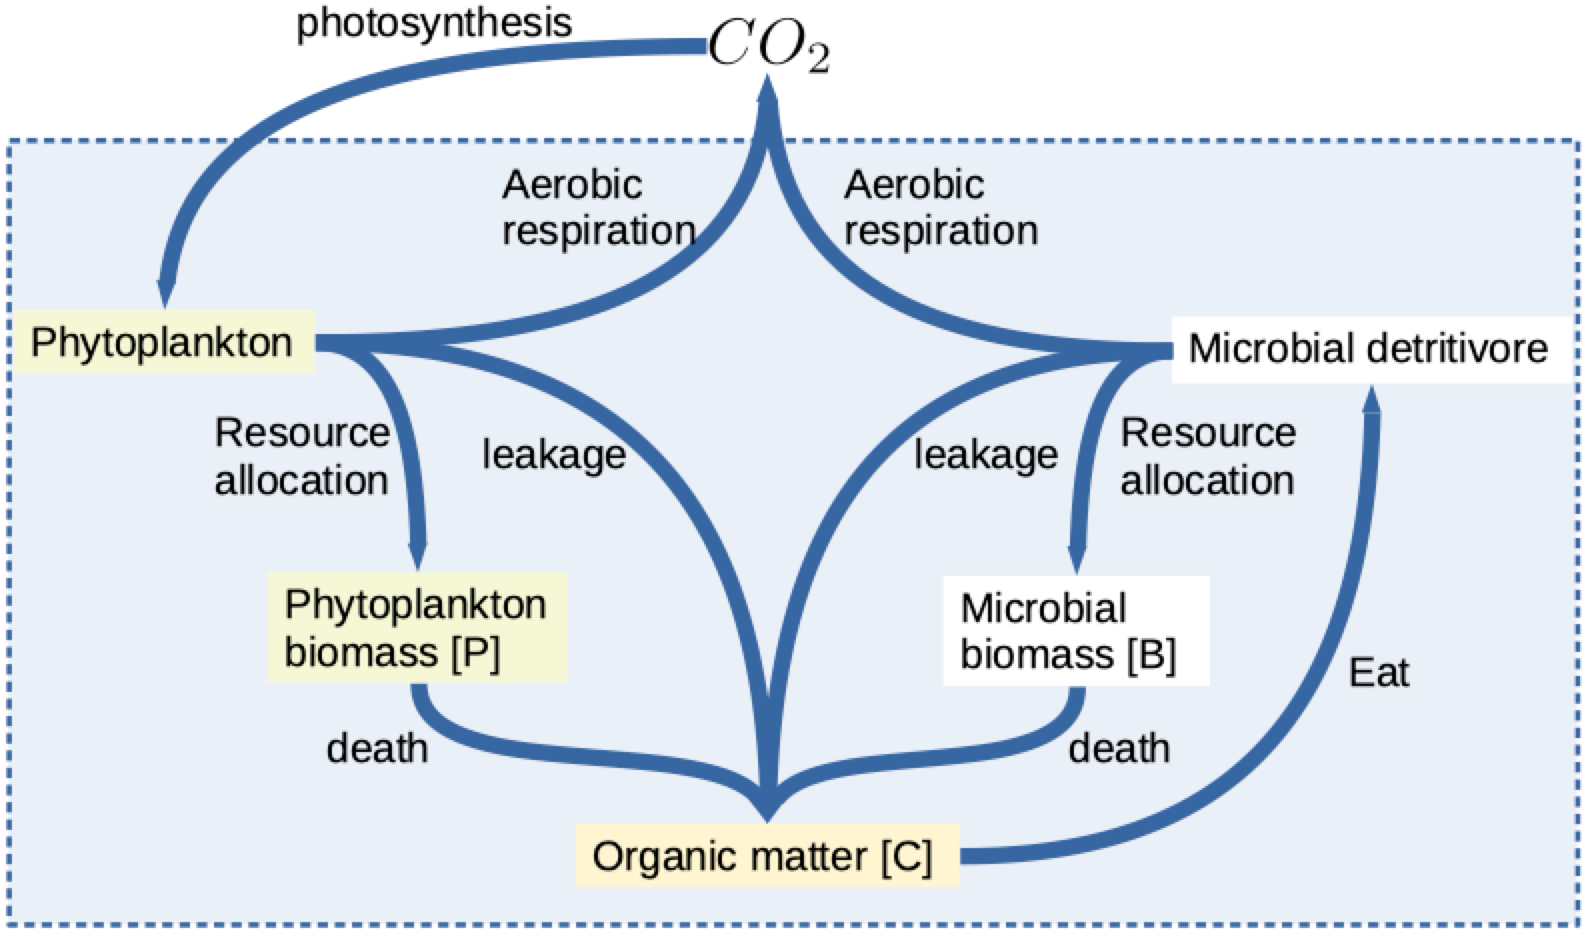
\includegraphics[width=.8\linewidth]{result/model.png}
    \caption[Model visualization]{Classification of dominant interactions in this project.  The two players shared all interactions with respective carbon pools but one, which was the energy acquiring method.}
    \label{modelInWord}
\end{figure}

In Fig.\ref{modelInWord}, players were sharing all but one linking methods to carbon pools, which was their carbon extraction pathway.  Phytoplanktons acquired carbon from external unlimited atmospheric carbon dioxide (CO$_2$) pool while detritivores gained carbon from finite C pool contributed from cellular leakages and remains upon death.  Both players carried out aerobic respiration and processed remaining portion of extracted carbon.  After carbon processed, a fraction of the portion was leaked from the cell (direct contribution to C pool) and the remaining part was incorporated into respective biomass carbon pool (either P or B pool).  Cellular death would release carbon from P and B pool to the C pool.  In the system, biomass pool (P and B) would logically be linked to carbon extraction power from food pools (either external CO$_2$ or C pool) directly because organisms were built from biomass.  Also, none of the pools can go to negative numbers because zero means a void pool.  However, there was not a upper boundary for any pools and the only limiting factor was the intraspecific interference (density-dependent) from phytoplanktons.

\subsection{Minimal ecosystem in an Ordinary Differential Equation (ODE) System}
The ecosystem described in Fig.\ref{modelInWord} can be translated to the following ODE system with the rate of change of carbon pool contents as subjects:

\begin{equation*}\left\{\begin{array}{rl}
    C'(t) &= (1-\varepsilon_P)\varepsilon_{PR}g_PP +a_PP^2 +g_BCB(e_{BR}(1-e_B)-1) +m_BB\\
    P'(t) &= \varepsilon_P\varepsilon_{PR}g_PP -a_PP^2\\
    B'(t) &= g_B\varepsilon_{BR}\varepsilon_{B}CB -m_BB
\end{array}\right.\end{equation*}

This was due to all microbial cell membranes were not impermeable to carbon compounds as measured.(REF)  So apart from metabolism (i.e. aerobic respiration) and resource allocated to maintenance and population growth there was a portion of resource leakage.  Cellular life also were finite, hence death had to be considered as carbon pool transfer from biotic (i.e. biomass) to abiotic (i.e. organic matter) pools.  Due to the difference in energy acquiring strategies, phytoplanktons could extract carbon dioxide (CO$_2$) externally but detritivores could only take carbon from finite C pool.

\end{document}
